\documentclass{article}
\usepackage{amsmath}
\usepackage{mathtools}
\usepackage{gensymb}
\usepackage[a4paper,inner=1.5cm,outer=1.5cm,top=2cm,bottom=0.5cm]{geometry} 
\usepackage{xcolor}
\usepackage{tikz}
\usepackage{multicol}
\usepackage{pgfplots}
\usetikzlibrary{intersections}
\usetikzlibrary{intersections,calc,angles,quotes}
\usetikzlibrary{calc,angles,positioning,intersections,quotes,decorations.markings}
\usepackage{tkz-euclide}
\usetikzlibrary{backgrounds}
\usetikzlibrary{calc,through}
\usetikzlibrary{angles}
\usetikzlibrary{fadings}
\usetikzlibrary{shapes.geometric}
\usetikzlibrary{shapes.symbols}
\usepackage{draftwatermark}
\usepackage{mathptmx}

\SetWatermarkText{\textcolor{black!30}{Mathema Shukur}}
\SetWatermarkFontSize{2 cm}
\usepackage[utf8]{inputenc}
\usepackage{fontspec}

\setmainfont{[Kalpurush.ttf]}
\newfontface{\en}{[Arial.ttf]} %%this is optional, if you want to use a secondary font. Any english font is supported
\newlength\Radius
\setlength\Radius{4cm}
\begin{document} 
	\Large
	\textcolor{red}{Welcome To} 
	\\
	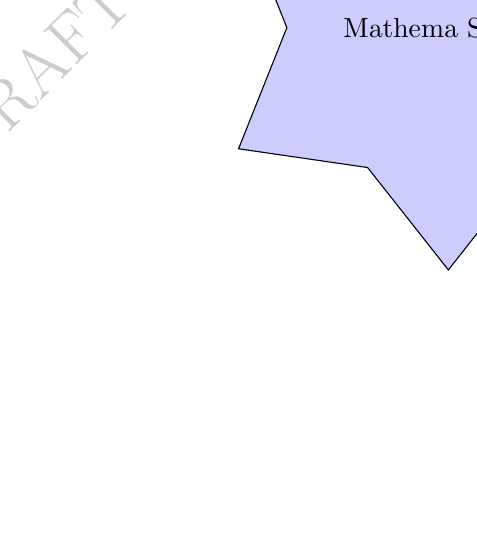
\begin{tikzpicture}
		\tikz \node [fill=blue!20,star,star points=6,draw] {Mathema Shukur };
	\end{tikzpicture}
	\\
	যাদের জন্যে প্রযোজ্যঃ  	\textcolor{magenta}{একাদশ ও দ্বাদশ শ্রেণীর শিক্ষার্থী} \\
	বিষয়ঃ \textcolor{magenta}{উচ্চতর গণিত ১ম পত্র} \\
	অধ্যায়ঃ \textcolor{magenta}{৩-সরলরেখা}\\ 
	Subtopicঃ  \textcolor{magenta}{ কার্তেসীয় ও পোলার স্থানাঙ্কের মধ্যে সম্পর্ক প্রতিষ্ঠা }\\
		\\
	\begin{tikzpicture}[transform shape,scale=1]
		\draw [-latex,thick](-3,0) -- (8,0) node[right] {$x$} coordinate(x axis);
		\foreach \x in {-3,-2,-1,1,2,3,4,5,6,7,8}
		\draw (\x,0.1) -- (\x,-0.1) node [fill=white,below] {$\x$};
		\draw [-latex,thick](0,-3) -- (0,8) node[above] {$y$} coordinate(y axis);
		\foreach \y in {-3,-2,-1,1,2,3,4,5,6,7,8}
		\draw (0.1,\y) -- (-0.1,\y) node [fill=white,left] {$\y$};
		\fill[black] (0,0) circle (1.5 mm);
		\fill[red] (4,4) circle (2 mm);
		\node[fill=white,above] at (4,4.2) {$\textcolor{red}{A(4,4)}$};
		\node at (4.2,-0.3) {$\textcolor{red}{C}$};
			\node at (-0.3,-0.3) {$\textcolor{red}{O}$};
		\node at (0.5,-0.5) {$\textcolor{purple}{(0,0)}$};
		\node at (1.3,0.4) {$\textcolor{blue}{45\degree}$};
		\draw[color=blue,ultra thick, ->] (1,0) arc (0:45:1cm);
		\draw[thick,red] (4,0)--(4,4);
		\draw[thick,red] (0,0)--(4,0);
		\draw[thick,blue] (0,0)--(4,4);
	\end{tikzpicture}
	\\
উপরের চিত্র অনুসারে কোনো একটি মটর সাইকেল $O$ বিন্দু থেকে $A$ বিন্দুতে যাওয়ার রাস্তা দুইটি \\
\\ 
	১ম রাস্তা (নীল)\\ 
	$O$ থেকে $x$ অক্ষের  ধনাত্মক দিকের সহিত $45\degree$ কোণে কোনাকোনিভাবে $4\sqrt{2}$ মিটার  দূরত্ব অতিক্রম করে $A$ বিন্দুতে পৌঁছায়। মোট ভ্রমণ দূরত্ব $4\sqrt{2}=5.7$ মিটার \\
	\\
	২য় রাস্তা (লাল)\\
$O$ থেকে অনুভুমিকভাবে $4$ মিটার দূরত্ব অতিক্রম করে $C$ তে পৌঁছায় তারপর উলম্বভাবে $4$ মিটার দূরত্ব অতিক্রম করে $A$ বিন্দুতে পৌঁছায়। মোট ভ্রমণ দূরত্ব $4+4=8$ মিটার \\ 
	\\
	মন্তব্য \\
	১ম রাস্তাটি পোলার স্থানাঙ্ক $(r,\theta)=(4\sqrt{2},45\degree)$ নির্দেশ করে\\
	\\
	২য় রাস্তাটি কার্তেসীয় স্থানাঙ্ক বা আয়তাকার স্থানাঙ্ক $(x,y)=(4,4)$ নির্দেশ করে\\
	\\
 ব্যবহারের দিক থেকে কার্তেসীয় স্থানাঙ্ক এর চেয়ে  পোলার স্থানাঙ্ক ব্যবস্থা উত্তম \\
 \\
 \begin{tikzpicture}[transform shape,scale=1]
 	\draw [-latex,thick](-3,0) -- (8,0) node[right] {$x$} coordinate(x axis);
 	\draw [-latex,thick](0,-3) -- (0,8) node[above] {$y$} coordinate(y axis);
 	\fill[black] (0,0) circle (1.5 mm);
 	\fill[red] (4,4) circle (2 mm);
 	\node[fill=white,above] at (4,4.2) {$\textcolor{red}{A(x,y)}$};
 	\node at (4.2,-0.3) {$\textcolor{red}{C}$};
 	\node at (-0.3,-0.3) {$\textcolor{red}{O}$};
 	\node at (0.5,-0.5) {$\textcolor{purple}{(0,0)}$};
 	\node at (2,-0.3) {$\textcolor{red}{x}$};
 	\node at (4.3,2) {$\textcolor{red}{y}$};
 		\node at (2.3,2) {$\textcolor{blue}{r}$};
 		\node at (1.3,0.4) {$\textcolor{blue}{\theta}$};	
 	\draw[color=blue,ultra thick, ->] (1,0) arc (0:45:1cm);
 	\draw[thick,red] (4,0)--(4,4);
 	\draw[thick,red] (0,0)--(4,0);
 	\draw[thick,blue] (0,0)--(4,4);
 \end{tikzpicture}
	\begin{multicols}{2}
			\begin{align*}
			\cos \theta&= \frac{OC}{OA}\\
			\\
			\cos \theta&= \frac{x}{r}\\
			\\
			x&=r\,\,\cos \theta\\
			&\boxed{x=r\,\,\cos \theta}
		\end{align*}
		\\
		\begin{align*}
			\sin \theta&= \frac{AC}{OA}\\
			\\
			\sin \theta&= \frac{y}{r}\\
			\\
			y&=r\,\,\sin \theta\\
			&\boxed{y=r\,\,\sin \theta}
		\end{align*}
	\end{multicols}
\begin{multicols}{2}
\begin{align*}
	&x^2+y^2\\
	\\
	&=(r\,\,\cos \theta)^2+(r\,\,\sin \theta)^2\\
	\\
	&=r^2\,\,\cos^2 \theta+r^2\,\,\sin^2 \theta\\
	\\
	&=r^2(\cos^2 \theta+\sin^2 \theta)\\
	\\
	&=r^2\\
	\\
	r^2&=x^2+y^2\\
	&\boxed{
	}
\end{align*}
\\
\begin{align*}
	\frac{y}{x}&=\frac{r\,\,\sin \theta}{r\,\,\cos \theta}\\
	\\
	\frac{y}{x}&=\tan \theta\\
	\\
	\tan \theta &=\frac{y}{x}\\
	&\boxed{\tan \theta =\frac{y}{x}}
\end{align*}
\end{multicols}
বিভিন্ন চতুর্ভাগে $\theta $ এর মান নির্ণয় \\
\\ 
\begin{tabular}{|c|c|c|}
	\hline
	১ম চতুর্ভাগে & $p(x,y)$ বিন্দুর জন্য & $\theta= \tan^{-1}|\frac{y}{x}|$\\
	\hline 
	২য় চতুর্ভাগে & $p(-x,y)$ বিন্দুর জন্য & $\theta= \pi - \tan^{-1}|\frac{y}{x}|$\\
	\hline
	৩য় চতুর্ভাগে & $p(-x,-y)$ বিন্দুর জন্য & $\theta= \pi+\tan^{-1}|\frac{y}{x}|,\quad \mbox{OR}\quad \theta= -\pi+\tan^{-1}|\frac{y}{x}| $\\
	\hline
	৪র্থ  চতুর্ভাগে & $p(x,-y)$ বিন্দুর জন্য & $\theta= 2\pi-\tan^{-1}|\frac{y}{x}|,\quad \mbox{OR}\quad \theta= -\tan^{-1}|\frac{y}{x}| $\\
	\hline
\end{tabular}
\\
(ঢাকা , চট্রগ্রাম, যশোর বোর্ড-২০২১)\\
$(-1,-\sqrt{3})$ বিন্দুটির পোলার স্থানাঙ্ক নির্ণয় কর \\ 
\\
$x=-1$,\quad $y=-\sqrt{3}$\\
\\
$r=\sqrt{x^2+y^2}=\sqrt{(-1)^2+(-\sqrt{3})^2}=\sqrt{1+3}=\sqrt{4}=2$\\
\\
বিন্দুটি ৩য় চতুর্ভাগে অবস্থিত \\
\\
$\theta= \pi+\tan^{-1}|\frac{y}{x}|,\quad \mbox{OR}\quad \theta= -\pi+\tan^{-1}|\frac{y}{x}| $\\
\\
$\theta= \pi+\tan^{-1}|\frac{-\sqrt{3}}{-1}|,\quad \mbox{OR}\quad \theta= -\pi+\tan^{-1}|\frac{-\sqrt{3}}{-1}| $\\
\\
$\theta= \pi+\tan^{-1}\sqrt{3},\quad \mbox{OR}\quad \theta= -\pi+\tan^{-1}\sqrt{3} $\\
\\
$\theta= \pi+\frac{\pi}{3},\quad \mbox{OR}\quad \theta= -\pi+\frac{\pi}{3} $\\
\\
$\theta=\frac{4\pi}{3},\quad \mbox{OR}\quad \theta= \frac{-2\pi}{3} $\\
\\
বিন্দুটির পোলার স্থানাঙ্ক $(r,\theta)=(2,\frac{4\pi}{3}),\qquad \mbox{OR}\quad (2,-\frac{2\pi}{3})$\\
\end{document}